\chapter{Implementação e resultados}
\label{cap:implementacaoresultados}

Neste capítulo será apresetado o projeto de implementação, detalhado a implementação com a configuração do \ac{OS}, do ambiente virtualizado e 
das ferramentas que irão compôr o \textit{cluster} de alta disponibilidade. Posteriormente, será apresentada a metodologia de testes e 
apresentado os resultados das medições para validação da alta disponibilidade.

\section{Implementação}
\label{section:implementacao}

O ambiente foi configurado na forma de um \textit{cluster}, o qual é composto por dois servidores com requisitos de configuração 
de 12 \textit{cores} de processamento, 14 GB de memória \ac{RAM} e 180 GB de disco rígido.
%real = 11 \textit{cores} de processamento, 12 GB de memória \ac{RAM} e 156 GB de disco rígido
Essa configuração inclui 2 GB de memória \ac{RAM} e 24 GB de disco para cada sistema operacional hóspede. Além disso, optou-se por utilizar o 
mesmo sistema operacional e o mesmo hipervisor que são adotados atualmente na empresa, o sistema \textit{Ubuntu 14.04 \ac{LTS}} e o \ac{KVM} 
\cite{kvm}, respectivamente. O detalhamento da instalação e configuração encontra-se no Apêndice \ref{ap:confos} e \ref{ap:confvirt}.

A estrutura física adotada está representada na Figura \ref{fig:projeto_fisico}. Pode-se observar os dois servidores ligados a um 
\textit{switch} através de dois cabos UTP, ou seja, cada servidor encontra-se conectado ao \textit{switch} através de dois cabos, de forma a 
implementar uma redundância do cabeamento.

\begin{figure}[h!]
 \centering
 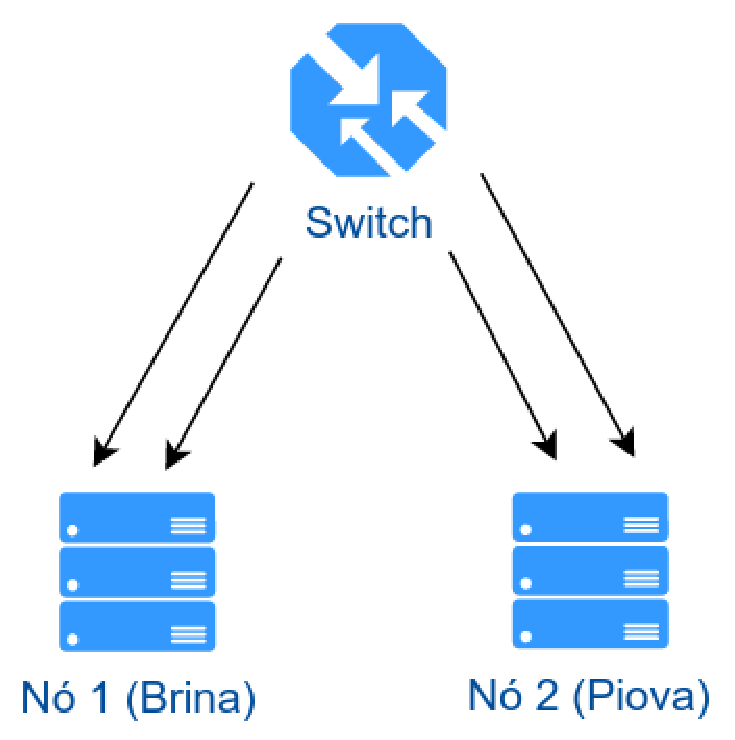
\includegraphics[width=180px]{img/projeto_fisico.eps}
 \caption{Estrutura física.}
 \label{fig:projeto_fisico}
\end{figure}

Para a configuração de rede manteve-se o \textit{link aggregation} e utilizou-se uma \textit{bridge} para incluir as máquinas virtuais à rede.
Os detalhes da configuração estão localizados no Apêndice \ref{ap:confrede}.

Na Figura \ref{fig:servidores_brina_piova} tem-se a imagem dos servidores, o primeiro é o \textit{Brina} (\textit{Dell PowerEdge 2950}), 
e o segundo servidor é o \textit{Piova} (\textit{Dell PowerEdge R410}).

\begin{figure}[h!]
 \centering
 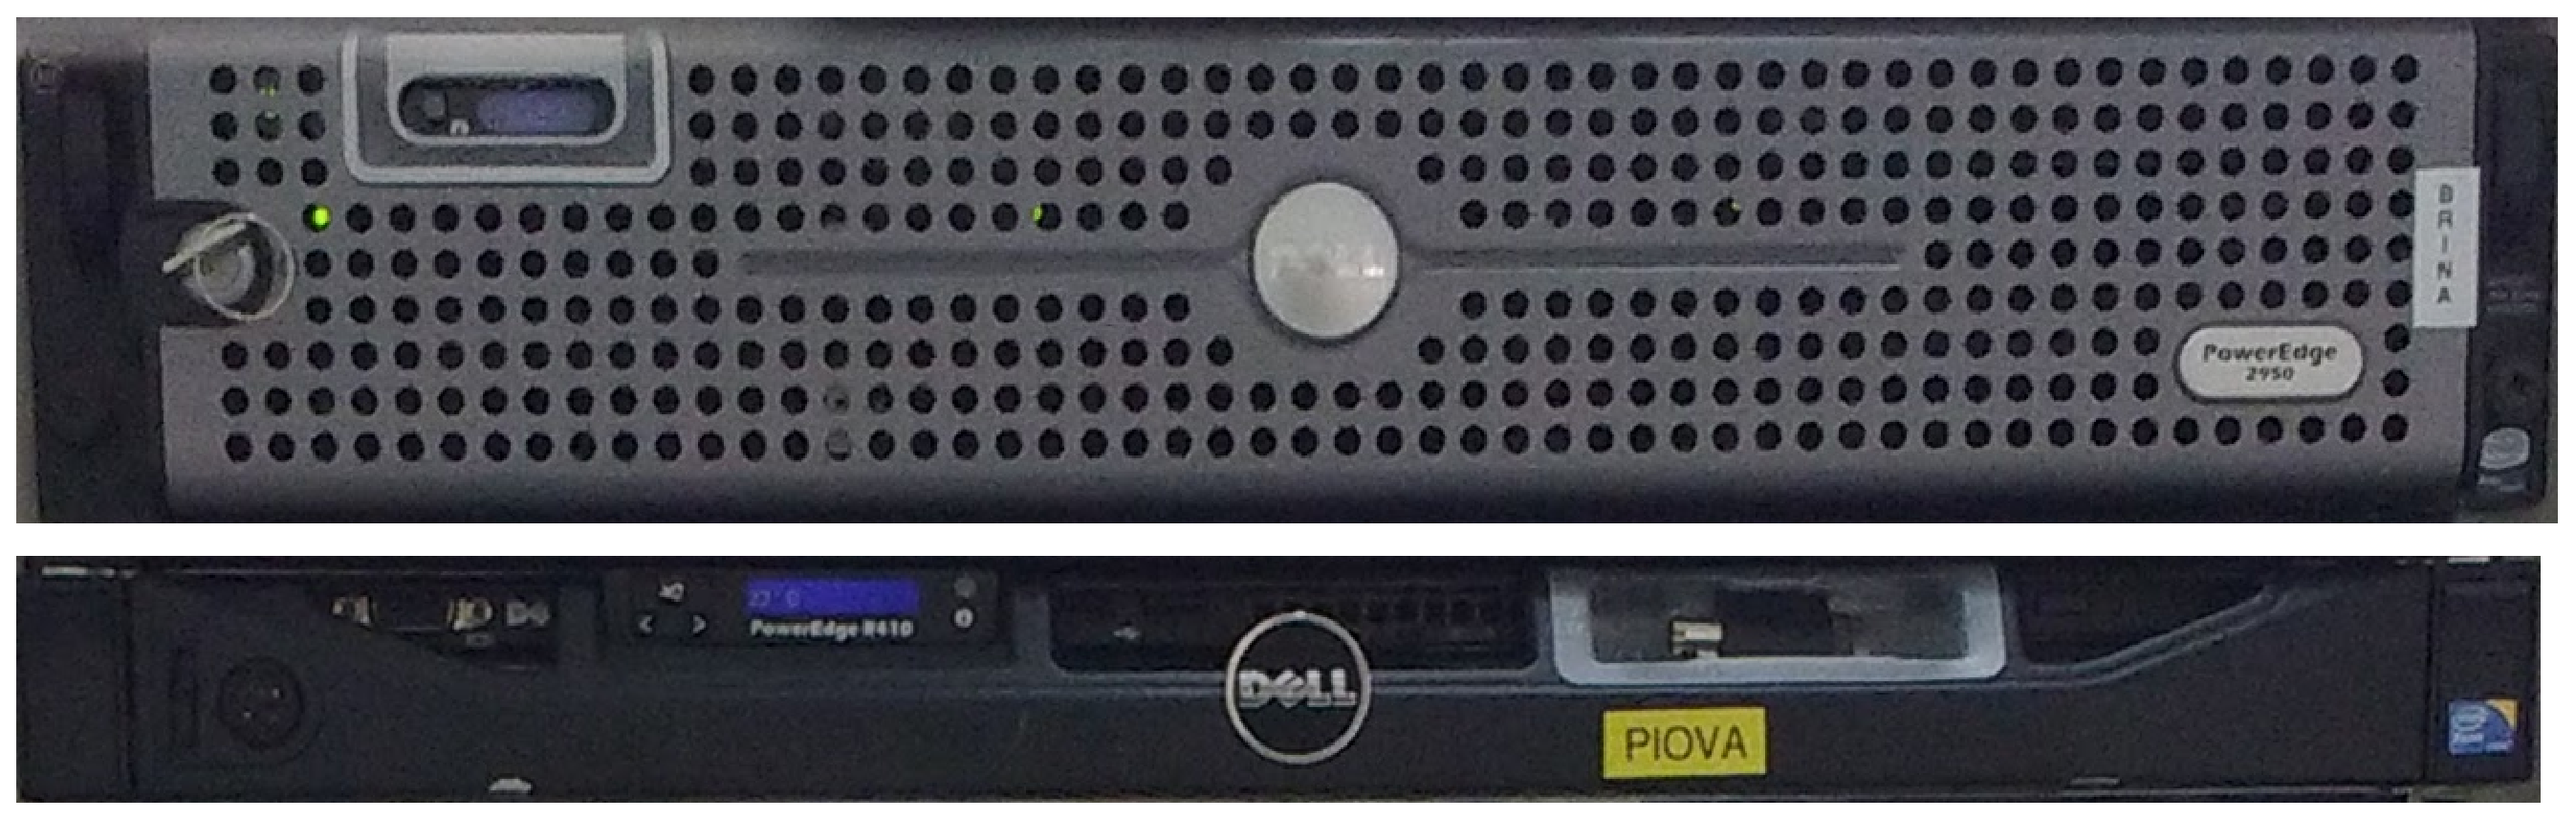
\includegraphics[width=300px]{img/servidores_brina_piova.eps}
 \caption{Servidores.}
 \label{fig:servidores_brina_piova}
\end{figure}

A estrutura lógica dos servidores juntamente com as máquinas virtuais e seus respectivos serviços são apresentados na Figura 
\ref{fig:projeto_estrutura}. Para a replicação de dados foi utilizado o \textit{software} \ac{DRBD}, que foi configurado no modo 
\textit{dual-master} onde os dois nós são configurados como primários. Para tal configuração é necessário utilizar um sistema de arquivos 
distribuídos que faz o gerenciamento do acesso aos dados, o \textit{software} adotado foi o \ac{OCFS2}. 
Os detalhes da instalação e da configuração de disco, \ac{DRBD} e sistema de arquivos estão detalhadas no Apêndice \ref{ap:confdisco}. 
O \textit{software} \textit{Pacemaker} faz o gerenciamento do \textit{cluster}, sendo responsável pela gerência, monitoramento e migração das 
\acp{VM} entre os nós.

\begin{figure}[h!]
 \centering
 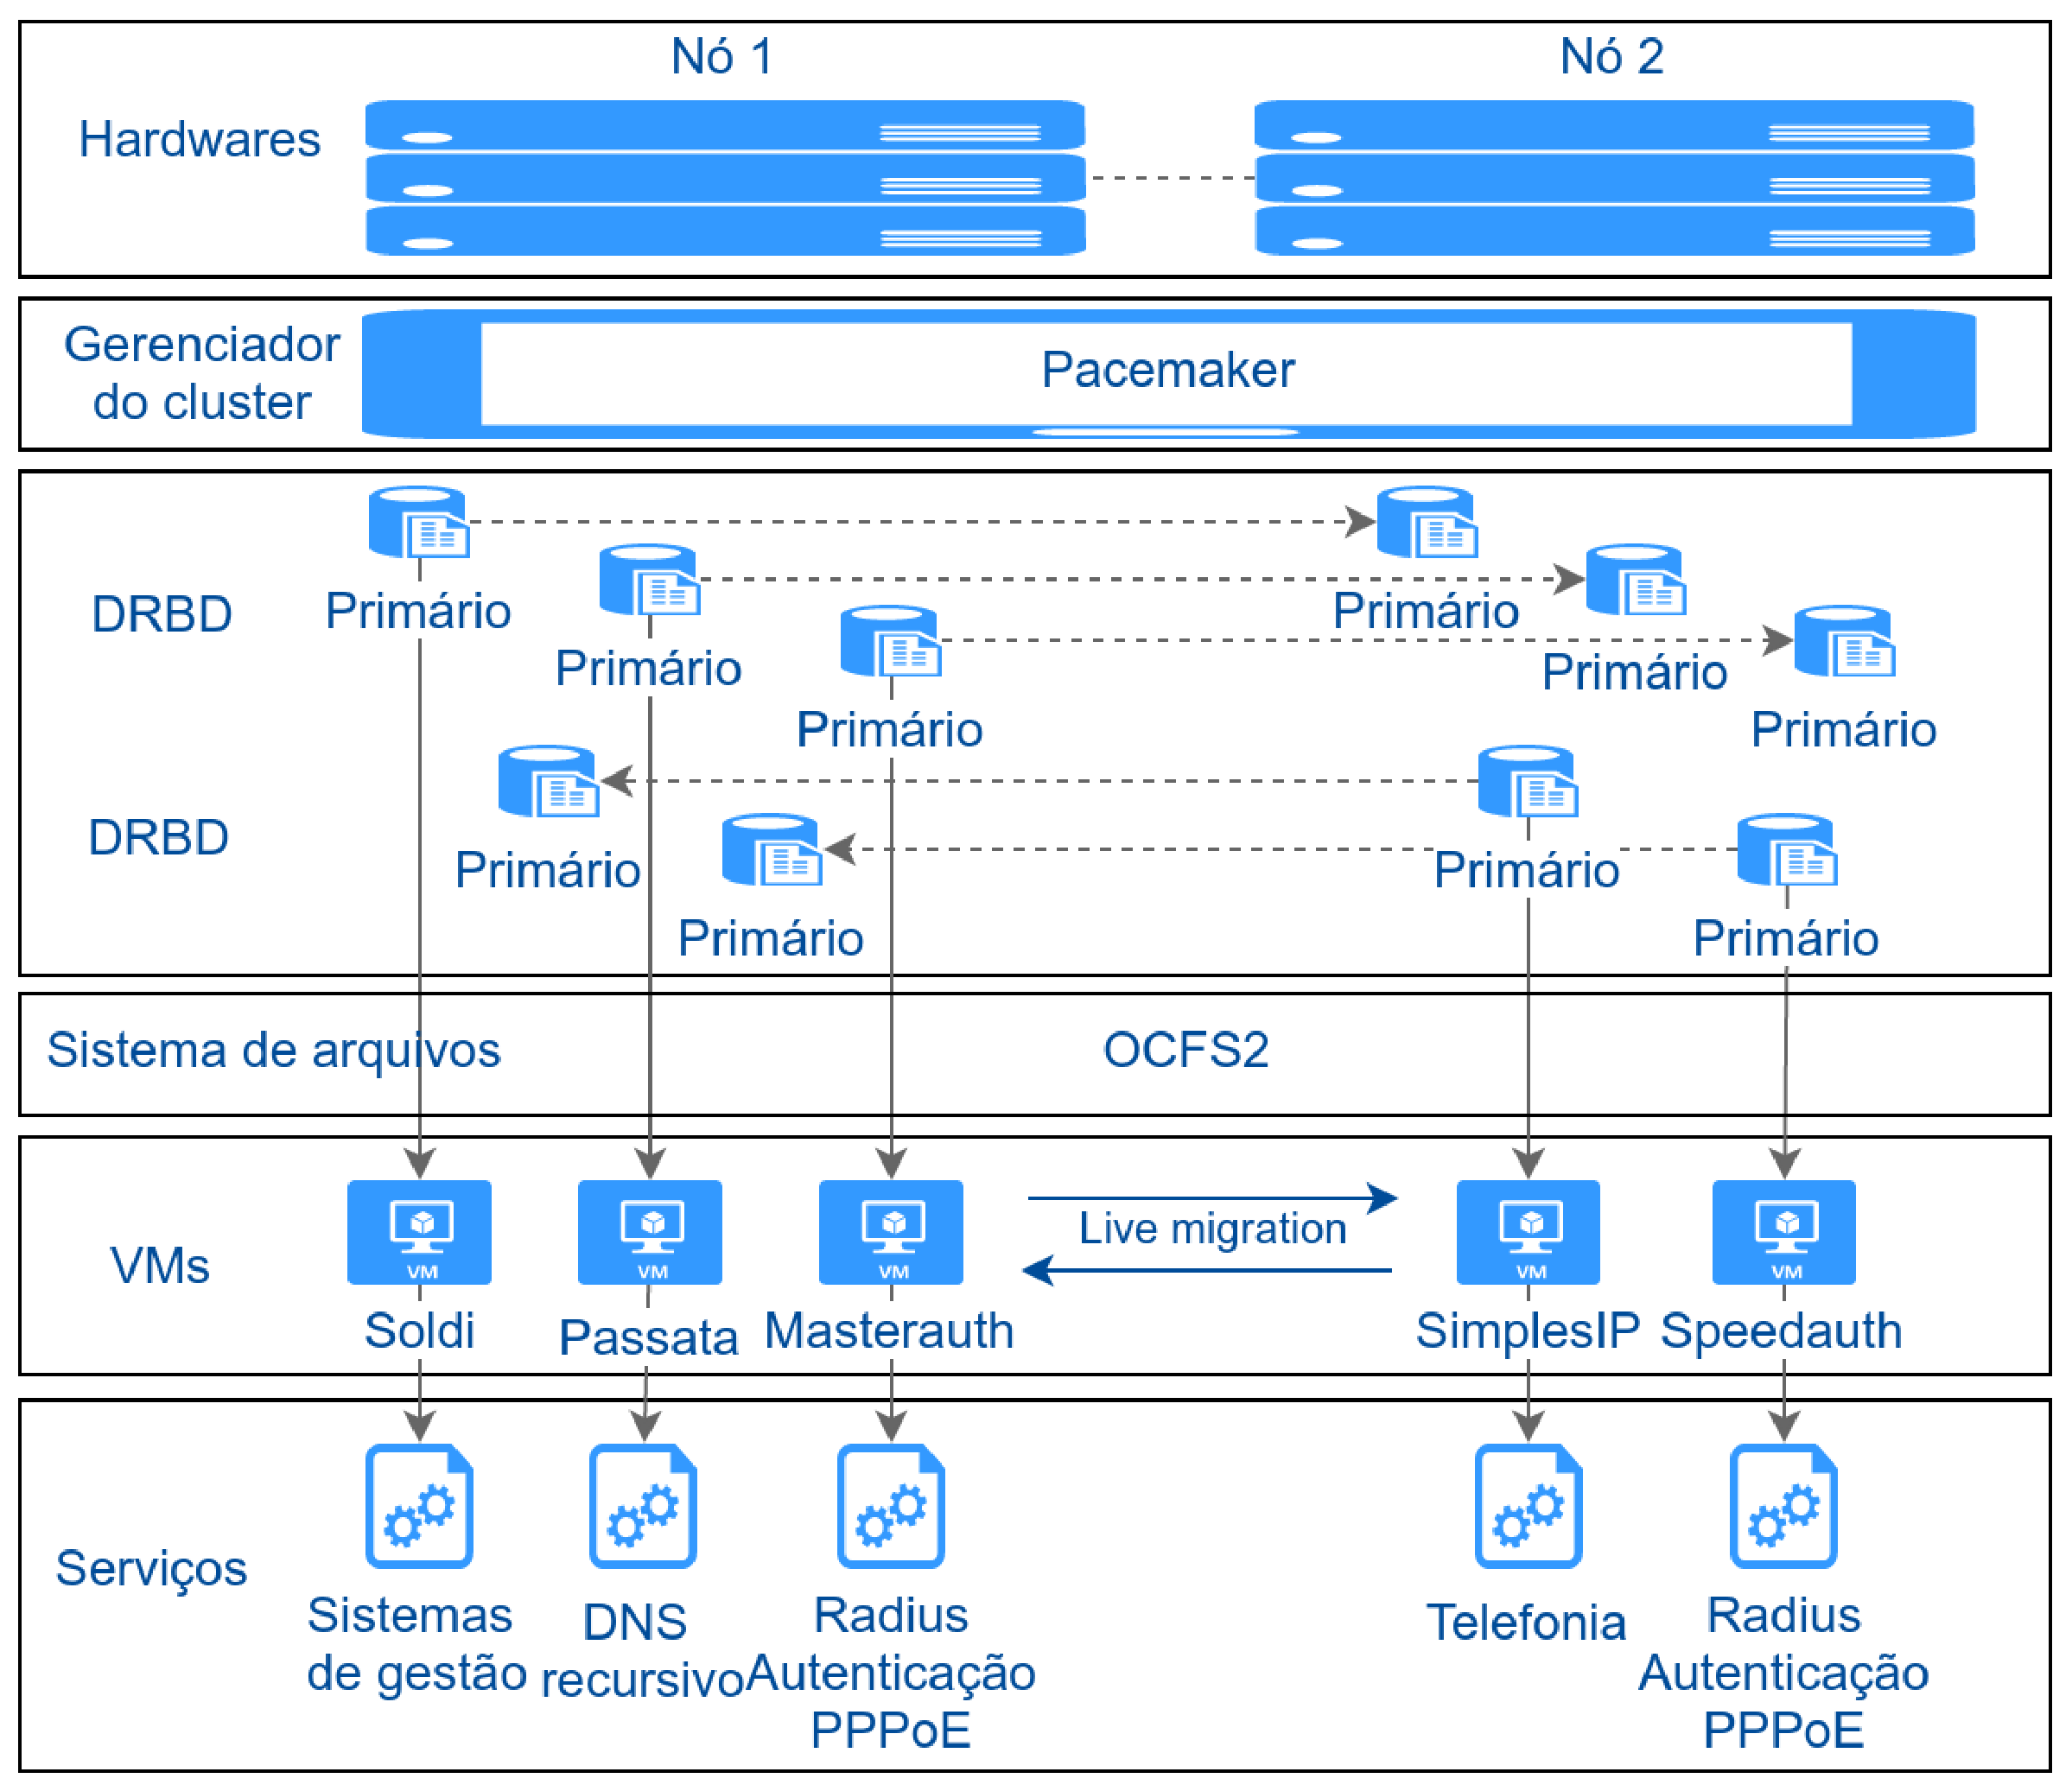
\includegraphics[width=350px]{img/projeto_estrutura.eps}
 \caption{Estrutura do \textit{cluster}.}
 \label{fig:projeto_estrutura}
\end{figure}

%drbd
% O \ac{DRBD} será configurado no modo \textit{master-slave}, sendo que para cada disco das máquinas virtuais será criado um dispositivo de 
% replicação \ac{DRBD}. E para utilizar esse dispositivo como disco de uma máquina virtual será criado um volume lógico 
% \ac{LVM}\footnote{LVM é uma ferramenta de código aberto que possibilita a manipulação de discos rígidos, através da criação de grupos de volumes 
% e volumes lógicos para \textit{Linux}.} \cite{lvm}. 

Deste modo, tem-se o ambiente pronto para a criação das \acp{VM}, sendo assim criou-se uma instância para cada servidor virtual. 
Como pode ser observado no Figura \ref{fig:projeto_estrutura}, criou-se três instâncias no Nó 1 e duas instâncias no outro Nó 2. De fato, o 
primeiro possui as instâncias dos servidores \textit{Soldi}, \textit{Passata} e \textit{Masterauth}. Já o segundo nó possui as instâncias dos 
servidores \textit{SimplesIP} e \textit{Speedauth}. Desta forma, quando houver uma falha em um nó, as instâncias serão iniciadas no nó disponível.
O detalhamento da configuração do \textit{Pacemaker} estão no Apêndice \ref{ap:confpacemaker}.


\section{Testes}
\label{section:testes}

Esta seção apresenta a metodologia de testes desenvolvida para ser possível analisar a eficácia do ambiente de alta disponibilidade.
... comprovar que o \ac{MTTR} é significativamente menor comparado a reconfiguração manual da \ac{VM}.
... objetivo também é comprovar que a gerência de falhas é importante para um ambiente, além de destacar que a gerência da manutenção também é 
favorecida através desta implementação.


Validação, metodologia de testes baseado nos trabalhos \cite{reis2009} e \cite{goncalves2009}:
-Desligamento físico (simulação falha de hardware ou eletrica): 4 vezes para medir tempo de downtime dos servicos e dos nodes (servico nao critico)
-Desligamento por software (reboot manual): 4 vezes para medir tempo de downtime dos servicos e dos nodes (servico nao critico)
-Agendamento de manutenção (reboot para atualização de software): 2 semanas ou mais, 1 manutenção por semana, com live migration, reboot e 
atualizacao de kernel dos nodes
-Medicao da disponibilidade dos serviços críticos por 1 mes (outubro) e comparar a mes setembro com uma reinicializacao dos servidores fisicos (reiniciados em 06/09)

Medição através do Nagios, que utiliza ping para calcular o tempo de downtime
Tabela com perda de pacotes, latencia, tempo de indisponibilidade

Fazer procedimento de teste para cada um, em itens

